\documentclass[twocolumn]{article}
\usepackage[pdftex]{graphicx}
\usepackage[cmex10]{amsmath}
\usepackage{caption}
\usepackage[font=footnotesize]{subfig}
\usepackage{url}
\usepackage{color}


% Additional packages added 2017 for the purpose of listing the license terms CC BY-SA
\usepackage[english]{babel}
\usepackage{hyperxmp}
\usepackage[hidelinks]{hyperref}
\usepackage{color}
\usepackage{fancyhdr}

\usepackage[
type={CC}, 
modifier={by-sa}, 
version={4.0},
lang={english},
imagewidth={45pt},
]{doclicense}

\pagestyle{fancy}
\lhead{}
\chead{}
\rhead{}
\lfoot{\begin{scriptsize} \doclicenseText \end{scriptsize} \\ 
\begin{Large}\ccbysa \end{Large} } 
\cfoot{\thepage}
\rfoot{}
\renewcommand{\headrulewidth}{0pt}

\begin{document}

\title{Improved Image Segmentation Through Energy Minimization Based
Subspace Fusion}

\author{David Kit Friedman\\
\href{https://github.com/davidkitfriedman}{\texttt{https://github.com/davidkitfriedman}}\\
\textit{Originally Written: 2007, Revised: Summer 2017}
}


\date{}
\maketitle

\thispagestyle{fancy}

\begin{abstract}

We discuss here an image segmentation scheme which combines multiple segmentations
from different subspaces. A subspace is any image characteristic which can help in 
segmentation, and in this paper we consider texture and intensity. Energy minimization via
graph cuts is used to fuse the intensity segmentation and the texture segmentation into a 
final segmentation. Previously published work used normalized cuts for the intensity 
segmentation algorithm and the texture segmentation algorithm. In this paper we 
investigate alternate algorithms for these steps in order to get better performance. 
We also propose a method to compute the quality input to the energy minimization 
algorithm more efficiently for a modified quality definition. The quality
computation involves an algorithm developed by the author for computing a 
measure of the variability within a particular window size 
throughout an image. 
\end{abstract}



\section{Introduction}

In image segmentation the goal is to divide the input into separate
logical components. In this paper we describe a segmentation scheme
based on \cite{prev}. Our scheme uses different internal algorithms and is
able to get better performance. We also show how it is possible to
execute the quality computation part of the algorithm more efficiently
for a modified quality definition. 

In the next section we discuss the scheme and in the section
after we discuss our results and make a few concluding
remarks. 

\section{Scheme}


\begin{figure}[!t]
\centering
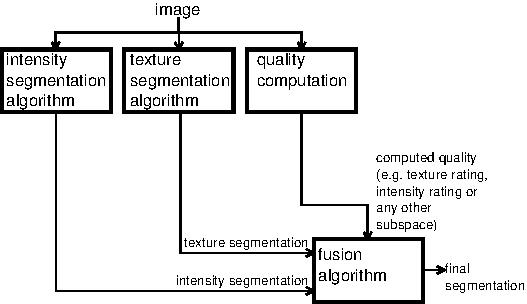
\includegraphics[width=3in]{overview}
\caption{Overview of the scheme}
\label{fig:overview}
\end{figure}


Fig. \ref{fig:overview} shows the basic components of the scheme. The
idea is to find segmentations in different subspaces and then to fuse
them to form a better total segmentation. A subspace could be any
particular characteristic of images that could help in
segmentation. In this scheme we consider texture and intensity. 


Sometimes an intensity segmentation will be better and sometimes
a texture segmentation will be better. For example, if the 
task is distinguishing between different animal furs a texture
segmentation will be more appropriate. On the other hand an intensity
segmentation would be more appropriate for distinguishing objects on a
desk. By taking information from both the intensity
segmentation and the texture segmentation one can get a
better total segmentation.

The quality computation is used to identify whether a particular image
region belongs to a particular subspace (e.g. whether it is intensity
or texture). The figure only shows a single box for the quality
computation, since the quality computation for texture and the quality
computation for intensity are computed in the same step, but in
principle there could be a separate metric and corresponding
computation for each separate subspace. \cite{prev} discusses some
additional possible subspaces. 

In the following sections we describe in more detail the
intensity segmentation algorithm \cite{intensity}, the texture
segmentation algorithm, the quality computation, and the
fusion algorithm \cite{fusion1}. An implementation is available at \url{https://github.com/davidkitfriedman/segment_fusion/}. 

\subsection{Intensity Segmentation}

The first step of the intensity algorithm \cite{intensity} 
is to form a graph from the image. Each pixel is a point and is 
connected to its immediate neighbors (including diagonally). 
The edge weight is the difference in intensity between the two
pixels. 

The next step is to sort all the edges from smallest to largest. The
algorithm then iterates through the edges and considers for each one
whether there is sufficient evidence between the two components to
join them. The algorithm takes into account the internal difference
within the components as well as the value of the edge
weight. Initially, each pixel is a single component. If the internal
difference within each component is small and the edge weight is large
then it will not join the two components as one would expect, but if
the edge weight is small in comparison to the internal difference it
will join them. One parameter of the algorithm is referred to as $k$
and sets the scale of observation. A larger $k$ will tend to favor
larger components, and a smaller $k$ will tend to favor more numerous
smaller components. More details on the exact criteria can be found in
\cite{intensity}.

Initially the algorithm will go through the smaller edges and there
will be more joins. At the end however it will be going through the
larger edges and there will be more non-joins. The algorithm is
completed after it has iterated through all the edges. 

The implementation of this algorithm was downloaded from 
\url{http://people.cs.uchicago.edu/~pff/segment/} (updated link
as of summer 2017: \url{http://cs.brown.edu/~pff/segment/}). 
The code used is also available in the source in its original
form.

\subsection{Texture Segmentation}

The first step of the texture segmentation algorithm is to find the
Fourier transform vectors. One of the parameters passed to the texture
segmentation algorithm is a window length. The image to be segmented
is divided into squares each containing 
$\mbox{window length} \times \mbox{window length}$ 
number of pixels, and the two dimensional Fourier
transform is taken of each of these windows. 

After the Fourier vectors have been found the next step is to
cluster them into separate textural segments. The previous
segmentation algorithm can be used if the Fourier vectors are
formed into a graph. In our implementation each vector is a
separate point and the edge weights between different points
is the sum of the absolute value of each coordinate
difference. 

It is possible to form the entire graph with all edges using
brute force. However, it is possible to get reasonable results
by only forming for each point the edge to its $k$
closest neighbors (in our implementation $k=5$
). Also, one can use a more efficient algorithm \cite{cell} than
brute force to find the nearest neighbors (as suggested in
\cite{intensity}). The previous segmentation algorithm can then be run on
this graph.  

We call our implementation of the algorithm described in \cite{cell}
the cell algorithm. The first step is to partition all of the
points into separate cells. The entire set is divided into two
parts based on the average value in the dimension of maximum
spread (\cite{cell} calls this the midpoint split rule). Each
subsequent set is recursively divided and the algorithm
continues until each cell has $bucket size$ or less
points in it.  

After the points have been split finding the nearest neighbors
involves iterating around the cells close to the query
point. Points are successively added to a point priority queue
which is prioritized based on how far the point is from the
query point. If a certain criteria is met then the closest
point is popped off the point priority queue and placed in a
result array which has $k$ slots for the result of
the search. The criteria is based on how far the current cell
is from the query point versus how far the point on the top of
the priority queue is from the query point. If the current
cell is distant from the query point then it is likely the
closest point(s) have already been encountered as the cells
are enumerated based on how far they are from the query
point. The parameter epsilon controls how fast versus how
precise the algorithm is. Fig. \ref{fig:cell} provides further
details. 

Testing showed that as epsilon decreases accuracy improves but runtime is
longer (as expected). Accuracy was measured by looking at the sum of the
distances to the 5 close neighbors found by the cell algorithm to the actual 5
closest neighbors found by brute force. In the case of epsilon equal to 50 the
percent in which the sum of the distances for the 5 close neighbors was within
10\% of the sum for the actual 5 closest neighbors went as 67.24\%, 57.33\%,
53.83\%, and 52.61\% for the four images (\texttt{car.ppm},
\texttt{friends.ppm}, \texttt{husky.ppm}, and \texttt{olympics2016.ppm}). In
the case of epsilon equal to 10 the accuracy improved so that it went as
94.71\%, 93.17\%, 91.61\%, 91.86\%; however, it is also the case that the
execution time increased going from 3s, 4s, 2s and 11s to 20s, 30s, 11s, and
38s. The default in the file is still set to epislon equal to 50. Comparing
the actual segmentations produced it is not clear that the theoretical
improvement in accuracy translates to better segmentations for the additional
time. It does seem to be the case though that for the \texttt{friends.ppm}
image and \texttt{olympics2016.ppm} there is more consolidation of
classifications (larger groups get larger and smaller groups get
smaller). This test and the output generated can be found in the source. 

\subsection{Quality Computation}

To compute the quality we follow the same approach as in \cite{prev},
and use the standard deviation as a measure of texture. That is, given
a particular window radius the standard deviation is taken for all
pixel values within that radius (or possibly less pixel values if the
center pixel is near an edge). This is done for each pixel so that
each pixel gets a different value. In the implementation we do not
take the square root so it is implemented to be the sum of the squares
of the differences from the mean divided by the total number of pixels
in the window.

Since this is done for each pixel it is clearly possible to
recompute the mean more efficiently than just readding each
time. When we move down a row $2R+1$ points are deleted and $2R+1$
points are inserted. It is only necessary to keep track of the
total sum and to subtract from it the values that are deleted
and to add to it the values that are inserted.  

Our implementation shows how it is possible to do a similar
thing for a modified definition of the variance. The change is
to simply consider instead the sum of the absolute value of
each difference from the mean. 

We now introduce some notation. The \texttt{below\_count} is the total number
of points below the mean. The \texttt{below\_sum} is the sum of the
differences of each below point from the mean. The \texttt{above\_count} and
\texttt{above\_sum} are defined similarly. It can also be helpful to visualize
the points on a one dimensional number line with the mean in the center. The
\texttt{above\_sum} and \texttt{below\_sum} are always positive so the sum of
these two (divided by the total number of points) is the desired quantity. A
transition point is a point that changes from being below the mean to above it
or from being above the mean to below it when the mean changes.

Clearly if there are no transition points then finding the new state
is not difficult. This will happen for example if there are many
points clustered close together to the left and many points clustered
close together on the right, and the mean simply gets shifted slightly
to the right. Then the \texttt{below\_count} and the
\texttt{above\_count} remain the same and the \texttt{below\_sum}
increases by \texttt{below\_count * (new\_mean - old\_mean)} while the
\texttt{above\_sum} decreases by \texttt{above\_count * (new\_mean - old\_mean)}.

However, if there are transition points it is necessary to account for
them. The discussion now follows the code in fig. \ref{fig:quality}. The
code shows the case for the mean increasing. The case for the mean
decreasing is similar. It is also necessary in the implementation to
handle points close to the edge.


\begin{figure}[!t]
\centering
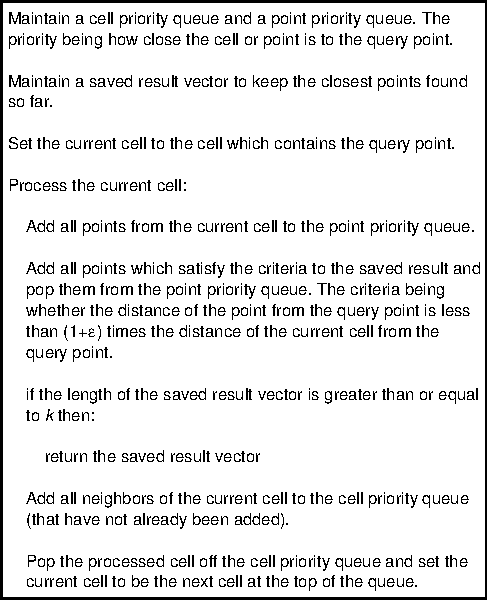
\includegraphics[width=3in]{cell}
\caption{Pseudocode for the cell algorithm}
\label{fig:cell}
\end{figure}



The first step is to find the transition points. For each transition
point that is found we increase the \texttt{below\_sum} by the
difference between the \texttt{new\_mean} and the current point. We
decrease the \texttt{above\_sum} by the difference between the current
point and the \texttt{old\_mean}. We also keep track of how many
transition points were found.

We then decrease the \texttt{above\_count} by the total number of
transition points and the \texttt{above\_sum} is decreased by
\texttt{above\_count*(new\_mean - old\_mean)}. 

We then increase the \texttt{below\_sum} by
\texttt{below\_count*(new\_mean - old\_mean)} and the
\texttt{below\_count} is increased by the total number of transition
points found.

After accounting for the additional points added to the set
the desired quantity is found by adding together the \texttt{below\_sum}
and the \texttt{above\_sum} and dividing by the total number of
points. The total number of points will increase at edges when
going toward the center and will decrease at edges when moving
away from the center, but in the middle will remain the same. 

It is also possible to do this without saving a lot of
state. By moving down each column it is only necessary to save
the state at the top of the column in order to transition from
one column to the next. It is only necessary then to keep
track of two states: the state for the previous pixel that was
just processed, and the state for the pixel at the top of the column.


\begin{figure}[!t]
\centering
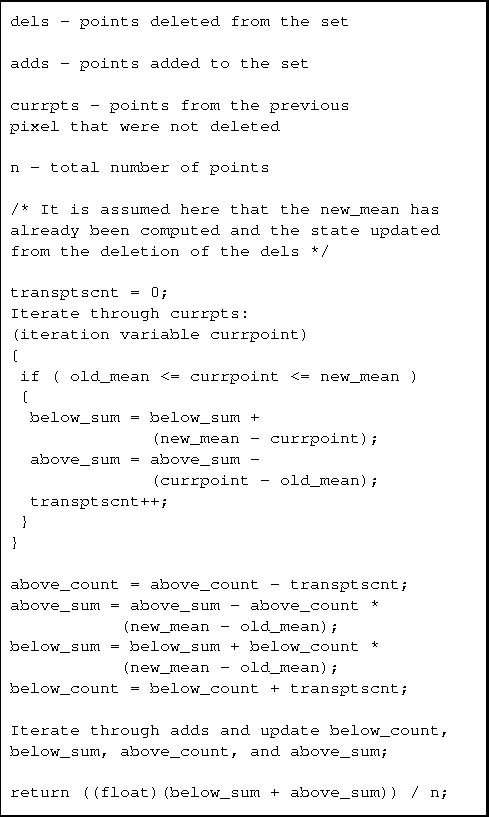
\includegraphics[width=3.15in]{quality}
\caption{Pseudocode for the quality computation}
\label{fig:quality}
\end{figure}


Experimental results indicate a performance improvement that
increases with the size of the window radius. It is not known 
whether a larger or a smaller window radius for the quality computation 
produces better segmentations. The source code for the tests and output fo
the testing machine can be found in the source.

\subsection{Fusion Algorithm}

In this step we have three inputs, the intensity segmentation, the
texture segmentation, and the quality computation. The objective is to
merge these two segmentations to produce a fused segmentation for the
whole image. 

\begin{figure*}[!t]
\centering
\subfloat[]{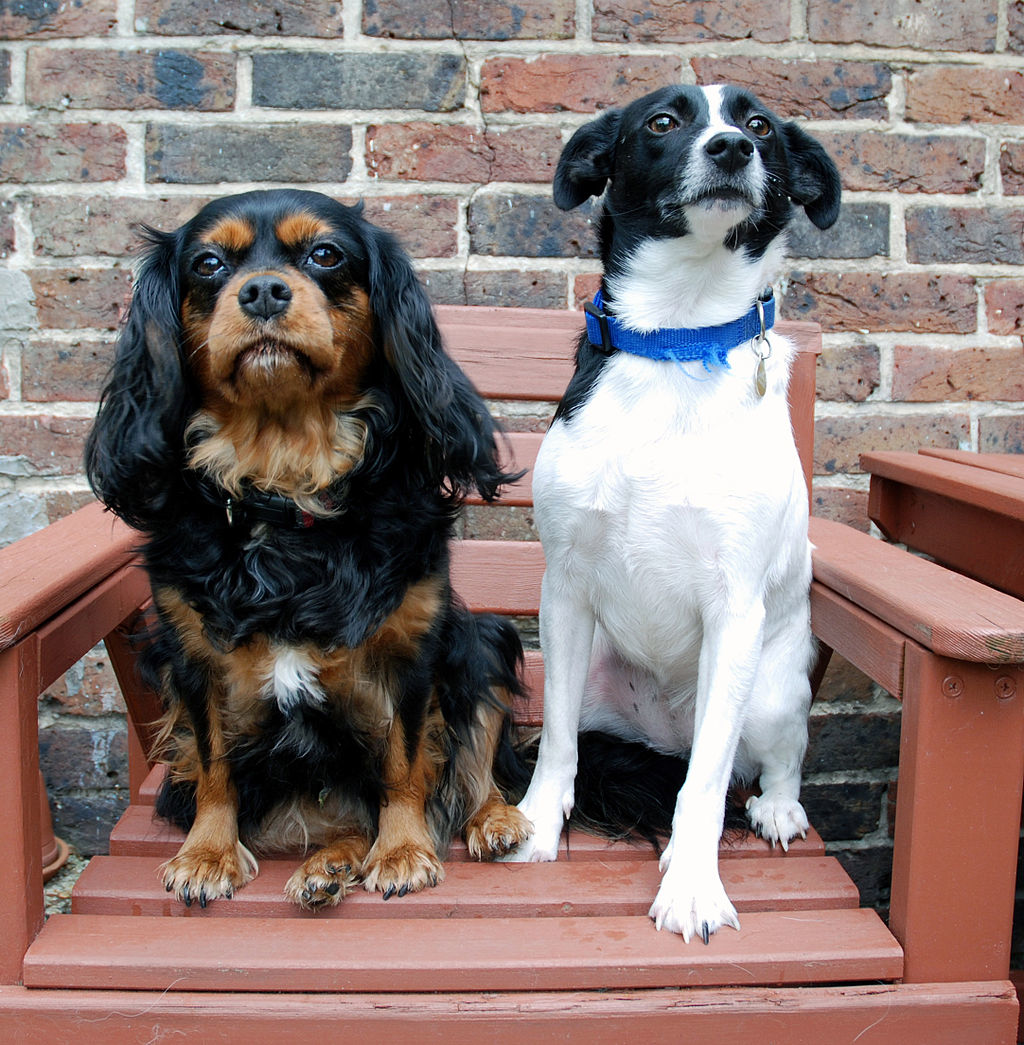
\includegraphics[width=2.5in]{friends.png}\label{fig:friends-pict}}
\hfil
\subfloat[]{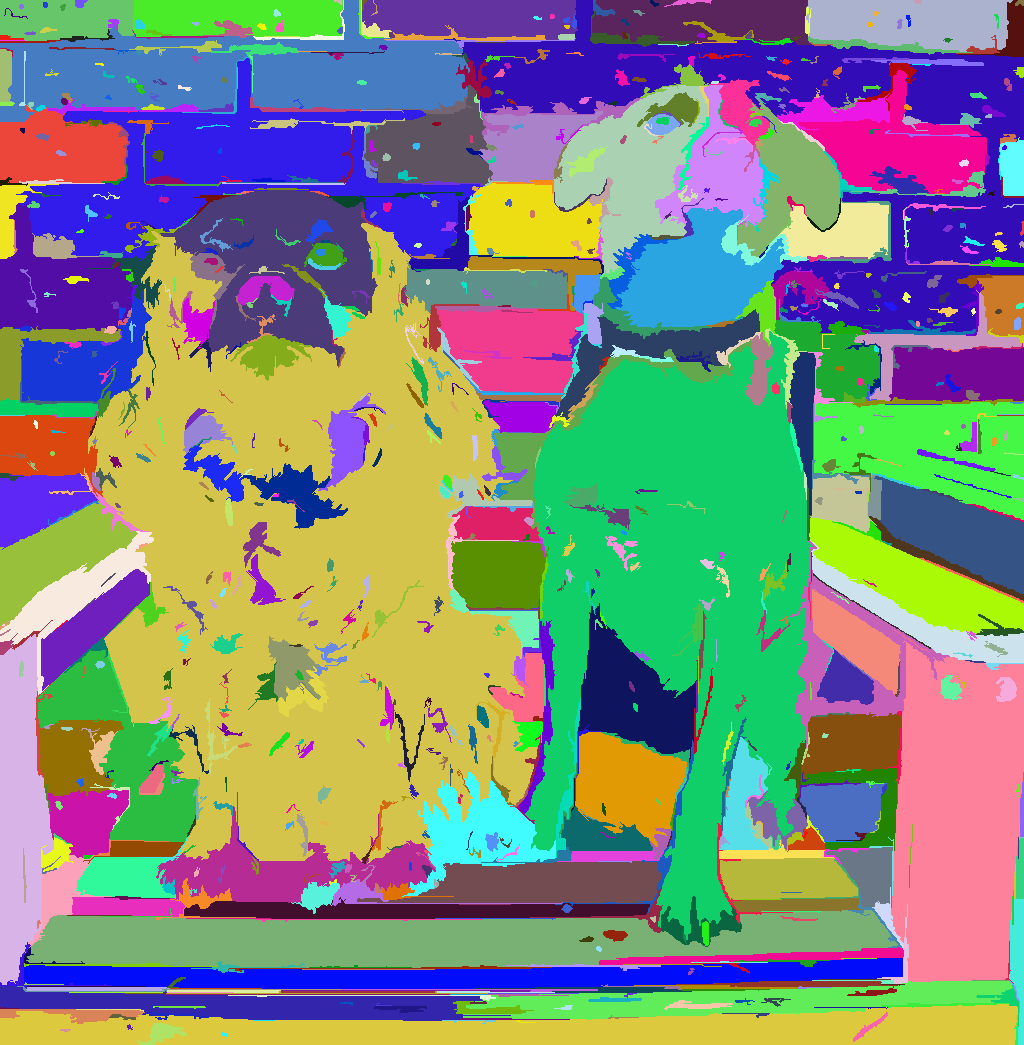
\includegraphics[width=2.5in]{friends_intensity.png}\label{fig:intensity-seg}}\\
\subfloat[]{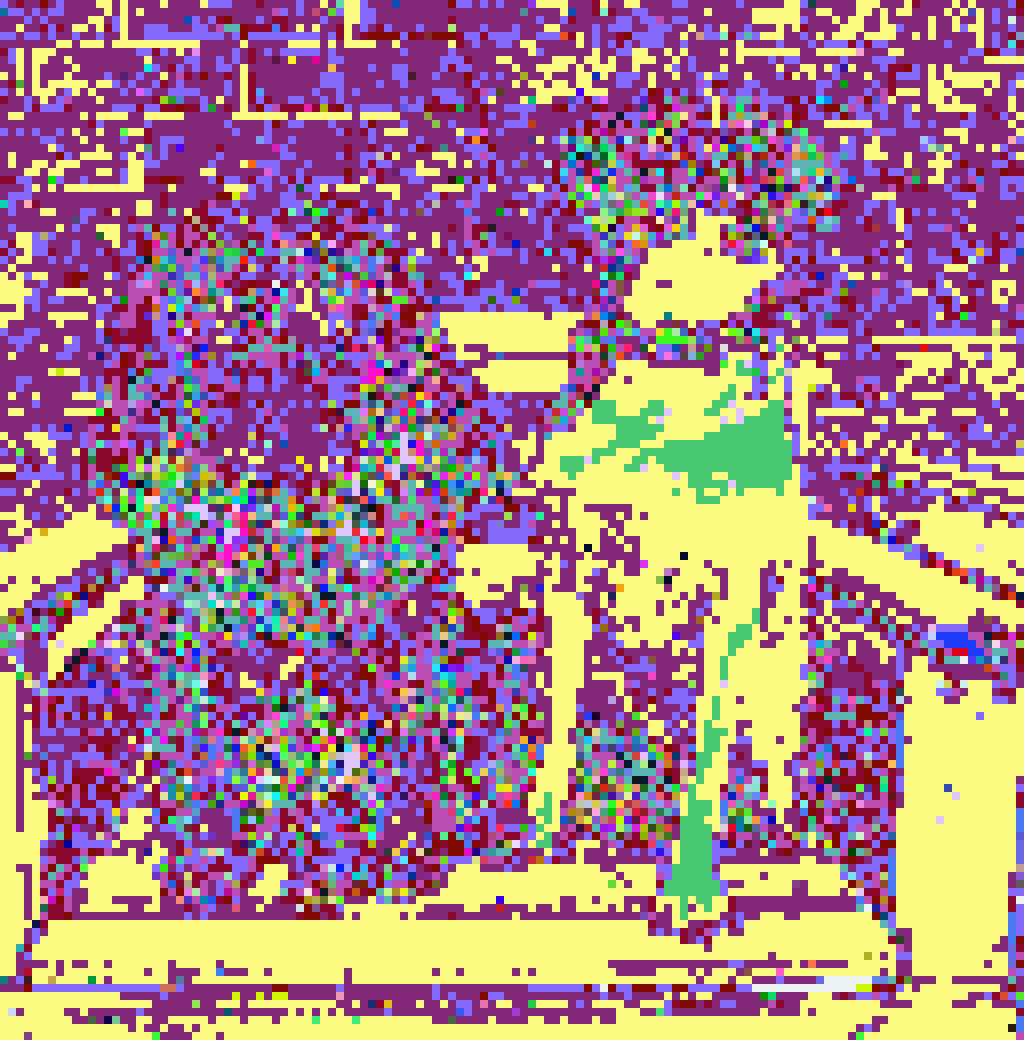
\includegraphics[width=2.5in]{friends_texture.png}\label{fig:texture-seg}}
\hfil
\subfloat[]{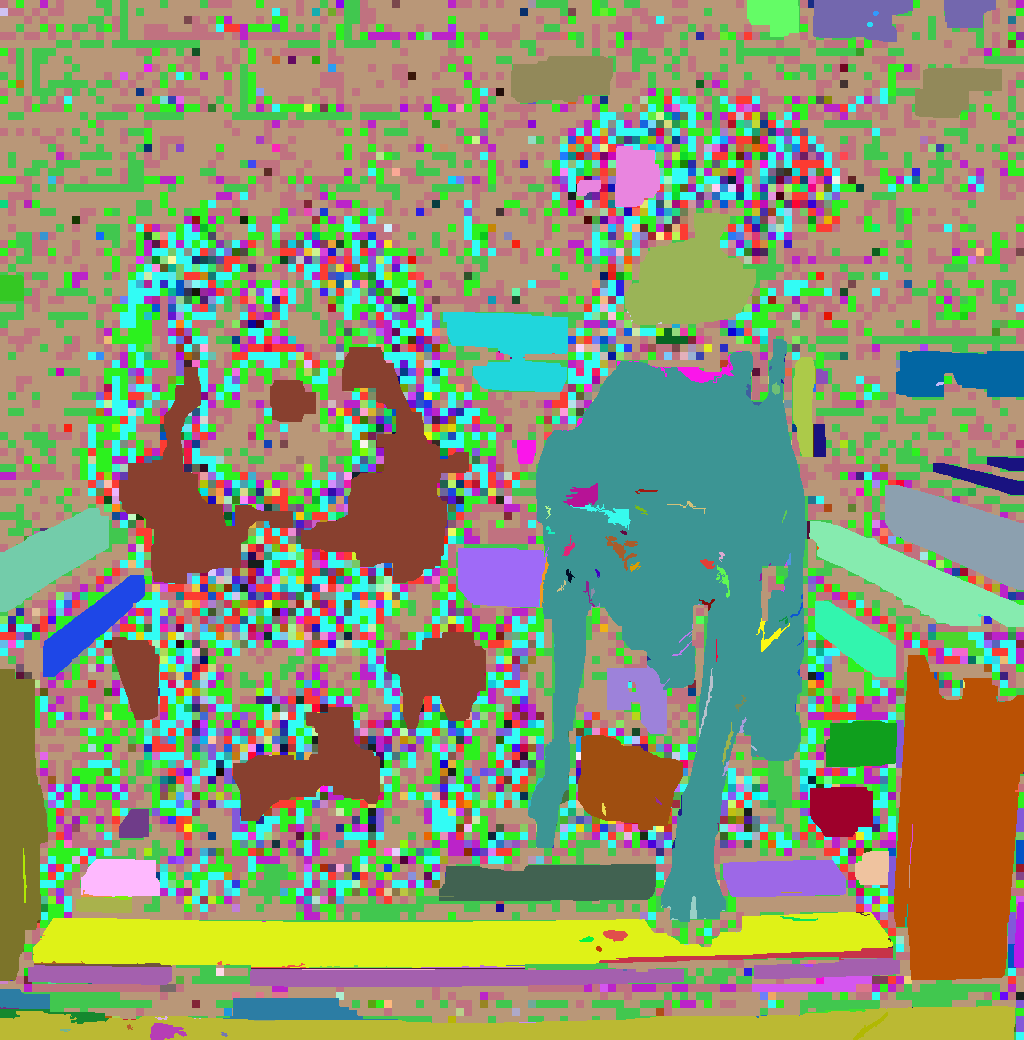
\includegraphics[width=2.5in]{friends_fused}\label{fig:fused-seg}}
\caption{(a) The original image (b) Intensity segmentation (c) Texture
Segmentation (d) Fused segmentation. The original image taken by 
\href{https://www.flickr.com/photos/allenthepostman/}
{\color{blue}Allen Watkin}
and posted on 
\href{https://www.flickr.com/photos/allenthepostman/3407703154/}
{\color{blue}Flickr} 
under a  
\href{http://creativecommons.org/licenses/by-sa/2.0}
{\color{blue}CC BY-SA 2.0} 
license 
\href{http://creativecommons.org/licenses/by-sa/2.0} 
{\ccbysa}
was downloaded from 
\href{https://commons.wikimedia.org/wiki/File\%3ABest_Friends_(3407703154).jpg}
{\color{blue}Wikimedia Commons}.
}
                              
\label{segs}
\end{figure*}

We have the quality computation which measures how likely a
region is to be intensity or texture. We could then just
produce a fused segmentation by using the texture segmentation
for each pixel that looks like texture and the intensity
segmentation for each pixel that looks like
intensity. However, this may not always be the best
approach. There might be a few pixels that look only slightly
more like texture than intensity within a larger region which
looks almost certainly like intensity. Those pixels may just
be noise or some object in the scene that will not be relevant
to a higher application. Instead of asking the question:
``does that pixel look like texture or intensity?'' it may be
better to ask the question: ``what arrangement of labels
(texture or intensity) best satisfies some specific
criteria?''. The criteria taking into account both the local
information and how well a particular label assignment fits
with other labels around it. 

This is a common problem in Computer Vision and the criteria
is typically called the energy. The objective is to minimize a
function of the following form: 
\begin{equation*}
 E = \sum_{p \in \mathcal{P}} D(p) + \sum_{p \text{ adjacent to } q} V(p,q)
\end{equation*}

$D(N)$ is the data cost and is over each pixel while $V(N)$ is the
smoothness cost and is over each pair of adjacent pixels. For example,
when doing stereo the data cost will be disparities, and the
smoothness cost will be some function which penalizes transitions
between different labels. In our case the labels are intensity and
texture, but for stereo the labels would be different distance
levels. 

There are multiple ways to approach this minimization problem
(although, in most cases there is no known way to get the
exact answer efficiently). This scheme models the problem as a
maximum flow minimum cut problem as done before in \cite{prev}. The
specific graph construction can be found in \cite{fusion1}. 

In our implementation the smoothness function used is: 

\begin{equation*}
V(p,q) = \begin{cases}
C&\text{ if $label(p)=label(q)$}\\
0&\text{ if $label(p) \neq label(q)$}\\
\end{cases}
\end{equation*}


which is referred to in \cite{fusion1} as the Potts model. The quality is
computed as described in the previous section. The intensity datacost
of a pixel is equal to the quality value at that pixel (lower variance
meaning more likely intensity). The texture datacost should be in same
way inversely related to the intensity datacost (higher variance
meaning more likely texture). In this scheme the additive inverse is
used so if the intensity datacost is $x$ the texture datacost is
$K-x$. However, setting $K$ to be the highest quality value found could lead
to everything be labeled as intensity since the highest quality value
found may be a large outlier, so $K$ is set to be the 75th percentile
quality value.    

All pixels labeled as intensity take the segment of the 
intensity segmentation and all pixels labeled as texture take the
segment of the texture segmentation. 

The code for this algorithm was downloaded from 
\url{http://www.csd.uwo.ca/~olga/code.html} (updated 
link as of summer 2017: \url{http://www.csd.uwo.ca/faculty/olga/code.html})
, and the version used for this implementation is also 
included in the source.   

\section{Results and Concluding Remarks}

Figs. \ref{fig:intensity-seg}, \ref{fig:texture-seg}, and \ref{fig:fused-seg}
show the results of the intensity segmentation,
texture segmentation, and fused segmentation for the image shown in
fig. \ref{fig:friends-pict}.

The variation in the bricks is large enough that those are considered texture
while the variation in the parts of the chair are small enough that the
intensity segmentation is used. The bricks are then composed of one principle
group with two smaller groups close in number. The variation in the coat of
the left dog is large enough that texture is used for most parts where about 
one one-fifth of the pixels have a texture classification also found in the
bricks. For the dog on the right the body has small enough variation that
intensity is used. 


The total amount of time taken to 
segment this image of size 1024 x 1045 was 22 seconds. Further images and 
segmentations can be found in the source.

Possible further work includes: 
\begin{itemize}

\item Improving the texture segmentation algorithm. Previously
\cite{prev} used Gabor convolution kernels \cite{gabor} so this could be
investigated in more detail. 

\item Considering alternate metrics for determining what part of
an image is texture versus what is not. 

\item Considering other subspaces as mentioned in \cite{prev}.

\end{itemize}

\section{Revisions made in 2017}

\begin{itemize}

\item The algorithm was run on new images for which the license information
  was readily available. Licensing issues were also addressed for the code,
  and licensing information was added to the paper and also in the source.

\item Consistent with new images the tests were rerun and the paragraphs in
  the paper reporting on the results of the tests were updated. 

\item In the course of testing a bug was fixed that would occur in the cell
  algorithm if all the pixel values were (0, 0, 0) resulting in a division by
  zero.

\item One paragraph related to testing was removed concerning absolute value
  and branching. The assembly produced for the testing machine did not use
  branching for absolute value and further investigation indicated that there
  are a variety of ways to avoid branching when doing absolute value. 

\item Various other revisions were made such as changes to formatting, etc.

\end{itemize}

\nocite{fusion2}
\nocite{fusion3}

\bibliographystyle{plain}
\bibliography{segment_fusion}


\end{document}


